\documentclass[10pt]{article}
\usepackage[polish]{babel}
\usepackage[utf8]{inputenc}
\usepackage[T1]{fontenc}
\usepackage{amsmath}
\usepackage{amsfonts}
\usepackage{amssymb}
\usepackage[version=4]{mhchem}
\usepackage{stmaryrd}
\usepackage{graphicx}
\usepackage[export]{adjustbox}
\graphicspath{ {./images/} }

\title{II Konkurs matematyczny St@ś }

\author{}
\date{}


\begin{document}
\maketitle
XIV LO im. Stanisława Staszica\\
29 maja 2002 roku

\section*{klasa V}
Na rozwiqzanie poniższych zadań masz 90 minut. Kolejność rozwiazywania tych zadań jest dowolna.\\
Wszystkie zadania sa jednakowo punktowane. Maksymalnq liczbę punktów może uzyskać jedynie pełne rozwiqzanie, z uzasadnieniem i odpowiedzia.\\
Uzywanie korektora i korzystanie z kalkulatora jest niedozwolone.

\section*{Zadanie 1.}
Podaj przykład dodatniej liczby naturalnej, której wszystkie cyfry są siódemkami lub zerami, i która dzieli się przez 75. Uzasadnij, zee podany przykład jest prawidłowy.

\section*{Zadanie 2.}
Za 15 lat Adam, Basia, Czarek i Dorota będą mieli razem 101 lat. Ile lat będą oni mieli razem za 5 lat?

\section*{Zadanie 3.}
Podaj przykład czterech różnych dodatnich ułamków dziesiętnych, których suma jest równa \(\frac{1}{8}\).

\section*{Zadanie 4.}
W pewnym trapezie suma kątów przy jednej podstawie jest dwa razy większa od sumy kątów przy drugiej podstawie. Jeden z kątów tego trapezu ma \(20^{\circ}\). Oblicz miary pozostałych kątów tego trapezu.

\section*{Zadanie 5.}
Na dwóch ścianach sześcianu narysowano szare kwadraty. Przerysuj siatkę tego sześcianu i zaznacz na niej drugi szary kwadrat.\\
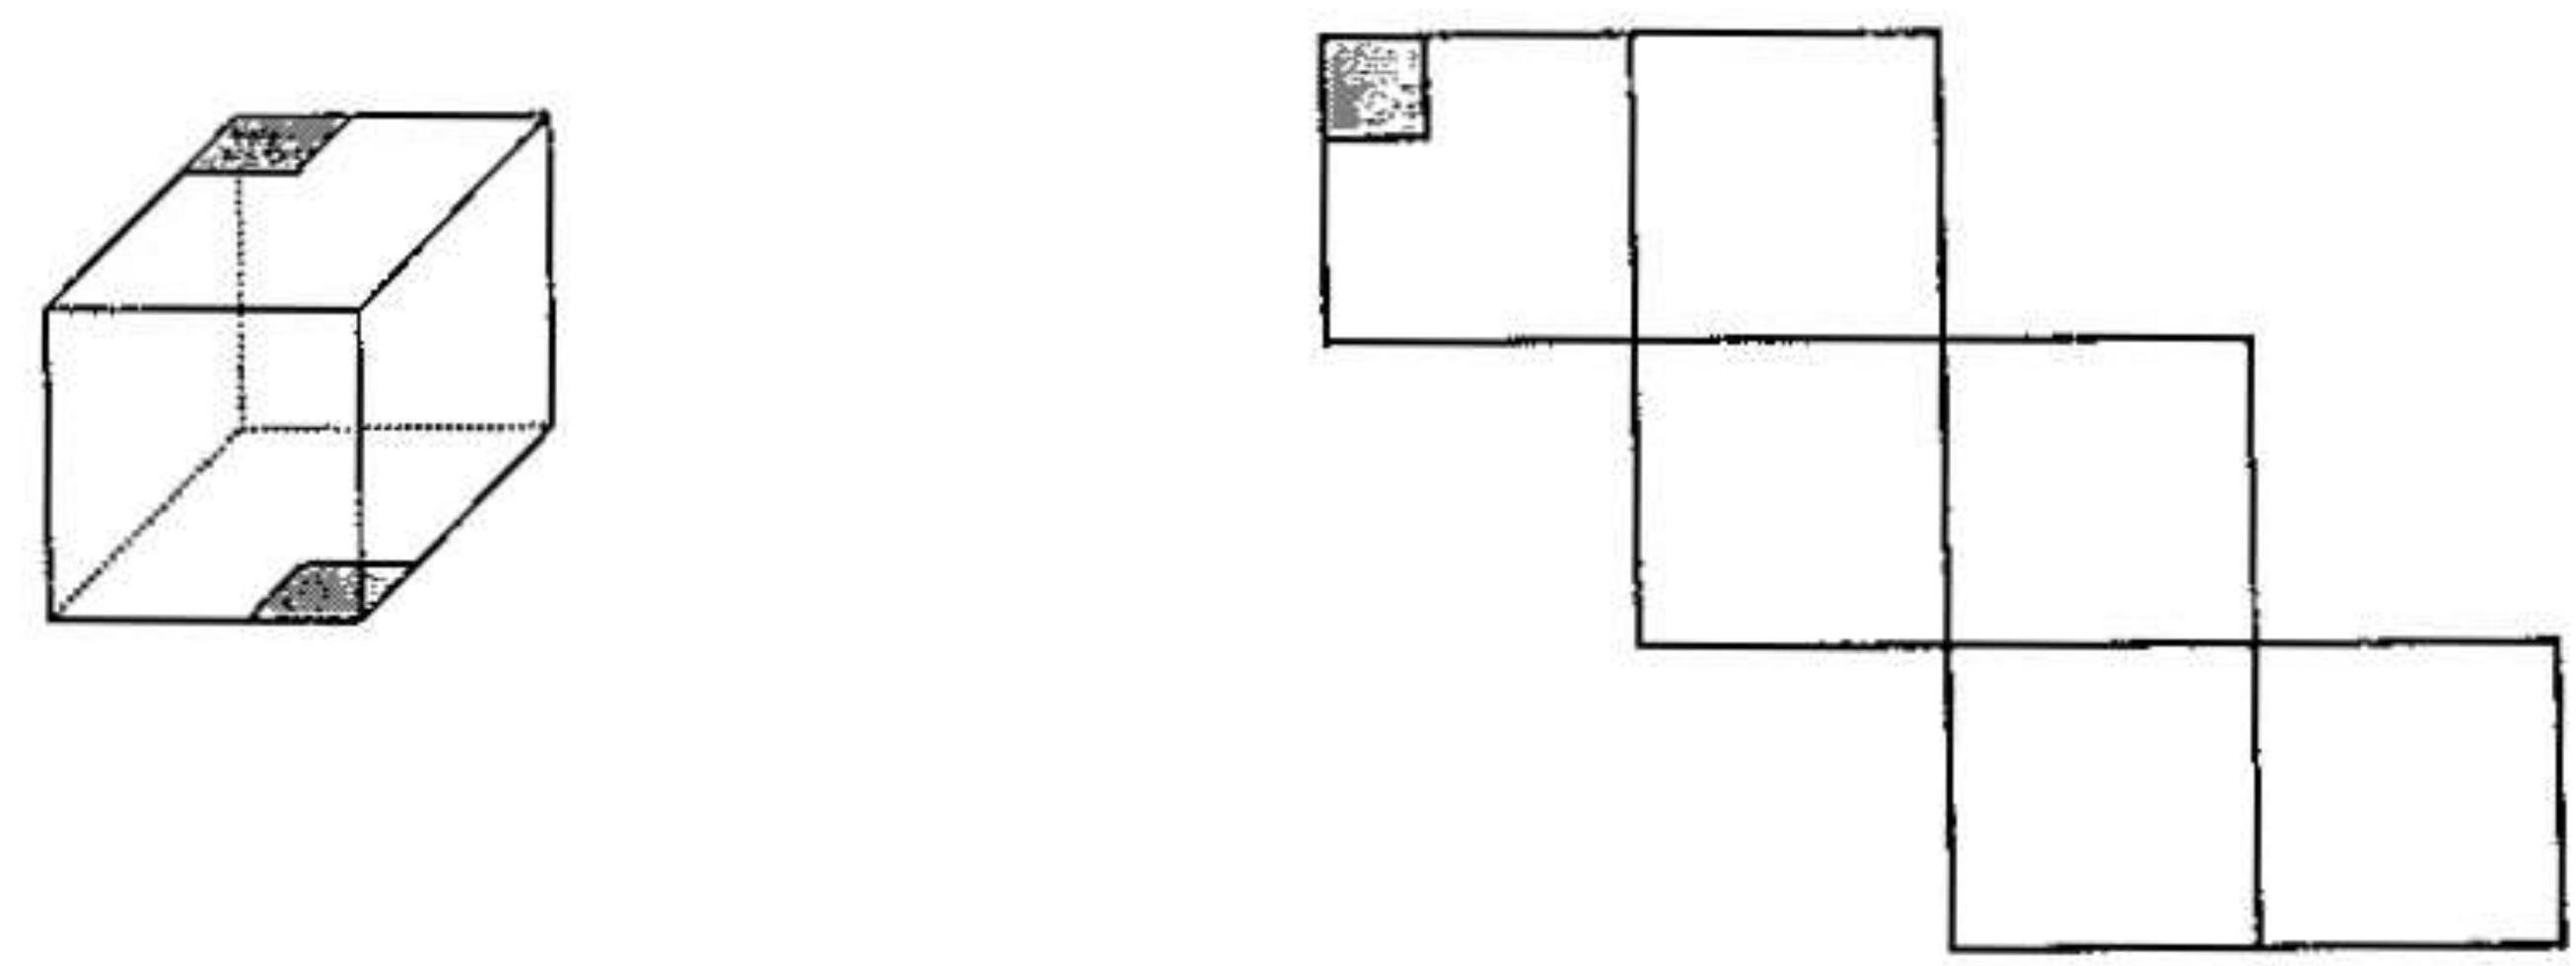
\includegraphics[max width=\textwidth, center]{2024_11_21_6040501f3d8f918315ffg-1}


\end{document}